\documentclass[8pt,executivepaper]{article}
\usepackage[utf8]{inputenc}
\usepackage[spanish]{babel}
\usepackage{amsmath}
\usepackage{amsfonts}
\usepackage{amssymb}
\usepackage{graphics}
\usepackage{graphicx}
\usepackage[left=1cm,right=1cm,top=2cm,bottom=2cm]{geometry}
\usepackage{imakeidx}
\makeindex[columns=3, title=Alphabetical Index, intoc]
\usepackage{listings}
\usepackage{xcolor}
\usepackage{multicol}
\usepackage{changepage}
\usepackage{float}
\usepackage{cite}
\usepackage{url}
\usepackage{hyperref}
\usepackage{pdfpages}
\usepackage{pgf,pgffor}
\usepackage{lscape}

\definecolor{codegreen}{rgb}{0,0.6,0}
\definecolor{codegray}{rgb}{0.5,0.5,0.5}
\definecolor{codepurple}{rgb}{0.58,0,0.82}
\definecolor{backcolour}{rgb}{0.95,0.95,0.92}
\lstdefinestyle{mystyle}{
    backgroundcolor=\color{backcolour},
    commentstyle=\color{codegreen},
    keywordstyle=\color{magenta},
    numberstyle=\tiny\color{codegray},
    stringstyle=\color{codepurple},
    basicstyle=\ttfamily\footnotesize,
    breakatwhitespace=false,
    breaklines=true,
    captionpos=b,
    keepspaces=true,
    numbers=left,
    numbersep=5pt,
    showspaces=false,
    showstringspaces=false,
    showtabs=false,
    tabsize=3
}
\lstset{style=mystyle}
\author{González Pardo Adrian}
\date{Junio 2020}
\title{Reporte ESCOMips Parte 1}
\newcommand\tab[1][1cm]{\hspace*{#1}}
\begin{document}
\maketitle
\section{Código de modulos de hardware}
\begin{center}
  \lstinputlisting[language=VHDL]{vhd/modulosHardware.vhd}
\end{center}
\section{Código de la arquitectura ESCOMips}
\begin{center}
  \lstinputlisting[language=VHDL]{vhd/escomips.vhd}
\end{center}
\clearpage
\section{RTL de la arquitectura}
\begin{center}
  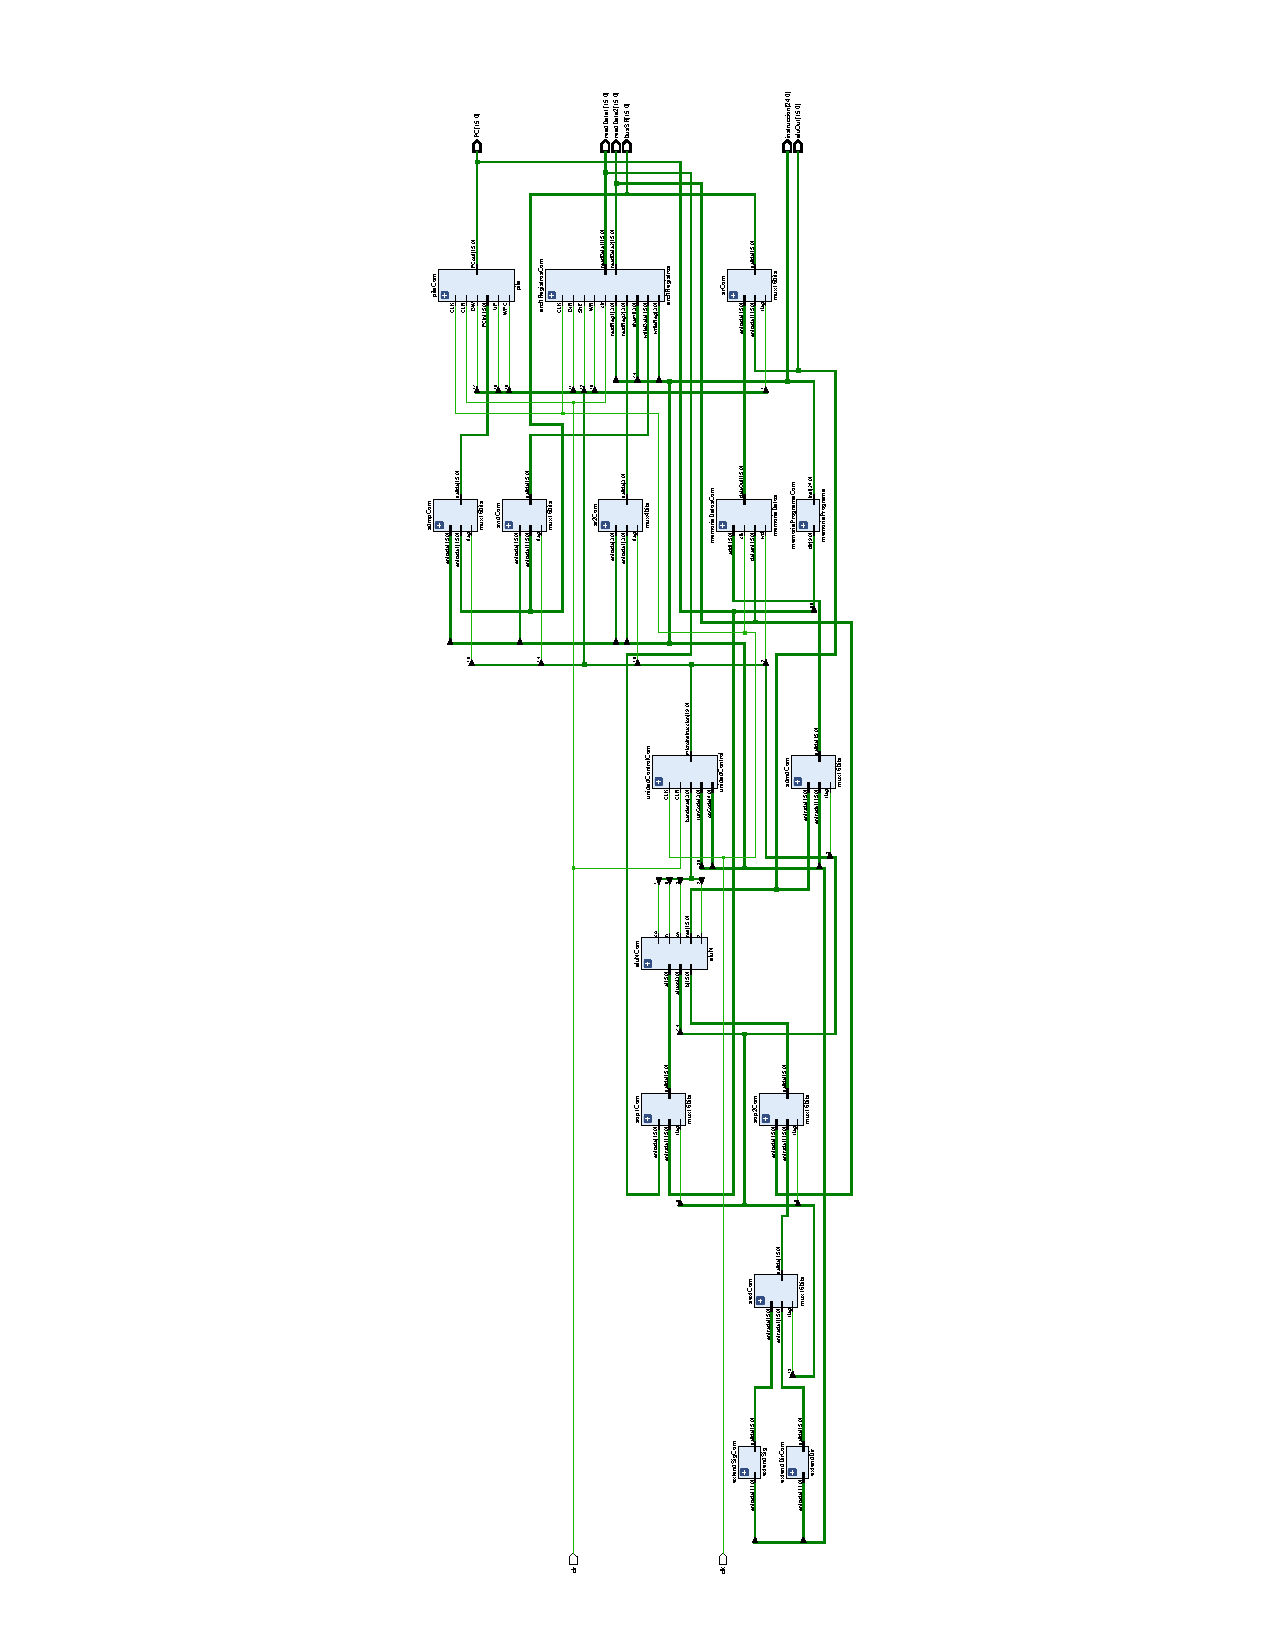
\includegraphics[scale=0.75]{rtl/escomips.pdf}
\end{center}
\section{Código del primer programa en Memoria de programa}
\begin{center}
  \lstinputlisting[language=VHDL]{vhd/programa1.vhd}
\end{center}
\section{Simulación imagenes}
\begin{center}
  \includegraphics[scale=0.35]{img/programa0-0.png}\\
  \includegraphics[scale=0.35]{img/programa0-1.png}
\end{center}
\begin{landscape}
  \section{Tabla del programa 1}
  \begin{tabular}{|c|c|c|c|c|c|c|c|c|c|c|c|}
    \hline
    Bus & T1 & T2 & T3 & T4 & T5 & T6 & T7 & T8 & T9 & T10 & T11\\
    \hline
    PC & 0000 & 0001 & 0002 & 0003 & 0004 & 0002 & 0003 & 0004 & 0002 & 0003 & 0004 \\
    \hline
    Instrucción & 0100001 & 0110007 & 0011000 & 0310005 & 1300002 & 0011000 & 0310005 & 1300002 & 0011000 & 0310005 & 1300002 \\
    \hline
    Read Data 1 & 0000 & 0001 & 0007 & 0001 & 0001 & 0008 & 0001 & 0001 & 0009 & 0001 & 0001\\
    \hline
    Read Data 2 & 0000 & 0001 & 0001 & 0008 & 0001 & 0001 & 0009 & 0001 & 0001 & 000a & 0001\\
    \hline
    Res ALU & 0000 & 0001 & 0008 & 0000 & 0001 & 0009 & 0001 & 0001 & 000a & 0000 & 0001 \\
    \hline
    Bus SR & 0000 & 0000 & 0008 & 0000 & 0000 & 0009 & 0008 & 0000 & 000a & 0009 & 0000\\
    \hline
  \end{tabular}
\end{landscape}
\section{Código del segundo programa en Memoria de programa}
\begin{center}
  \lstinputlisting[language=VHDL]{vhd/programa2.vhd}
\end{center}
\section{Simulación imagenes}
\begin{center}
  \includegraphics[scale=0.35]{img/programa1-0.png}
\end{center}
\begin{landscape}
  \section{Tabla del programa 2}
  \begin{tabular}{|c|c|c|c|c|c|c|c|c|c|c|c|}
    \hline
    Bus & T1 & T2 & T3 & T4 & T5 & T6 & T7 & T8 & T9 & T10 & T11\\
    \hline
    PC & 0000 & 0001 & 0002 & 0003 & 0004 & 0005 & 0006 & 0007 & 0008 & 0004 & 0005 \\
    \hline
    Instrucción & 0100000 & 0110001 & 0120000 & 013000f & 0040100 & 0601000 & 0614000 & 0522001 & 0f32ffc & 0040100 & 0601000 \\
    \hline
    Read Data 1 & 0000 & 0000 & 0000 & 0000 & 0000 & 0001 & 0001 & 0000 & 0001 & 0001 & 0001\\
    \hline
    Read Data 2 & 0000 & 0000 & 0000 & 0000 & 0001 & 0000 & 0001 & 0001 & 000F\&0000 & 0001 & 0001\\
    \hline
    Res ALU & 0000 & 0000 & 0000 & 0000 & 0001 & 0001 & 0001 & 0001 & FFF2\&0004 & 0002 & 0001 \\
    \hline
    Bus SR & 0000 & 0000 & 0000 & 0000 & 0001 & 0001 & 0001 & 0001 & 0000\&0004 & 0002 & 0001 \\
    \hline
  \end{tabular}
\end{landscape}
\end{document}
